\chapter{Transformer Architecture}

Transformers \cite{attention_is_all_you_need} were proposed by Vaswani et al. in 2017. This novel architecture achieved state-of-the-art results in machine translation tasks, while dispensing with recurrent and convolutional architectures, which enabled parallelization and speedup of natural language processing tasks.The Transformer employs an encoder-decoder stack, each with multiple \emph{blocks}, as can be seen in \ref{fig:transformer}. The key mechanism behind this architecture is called \emph{attention}, which we will discuss in detail in a later section.

\begin{figure}[h]
    \centering
    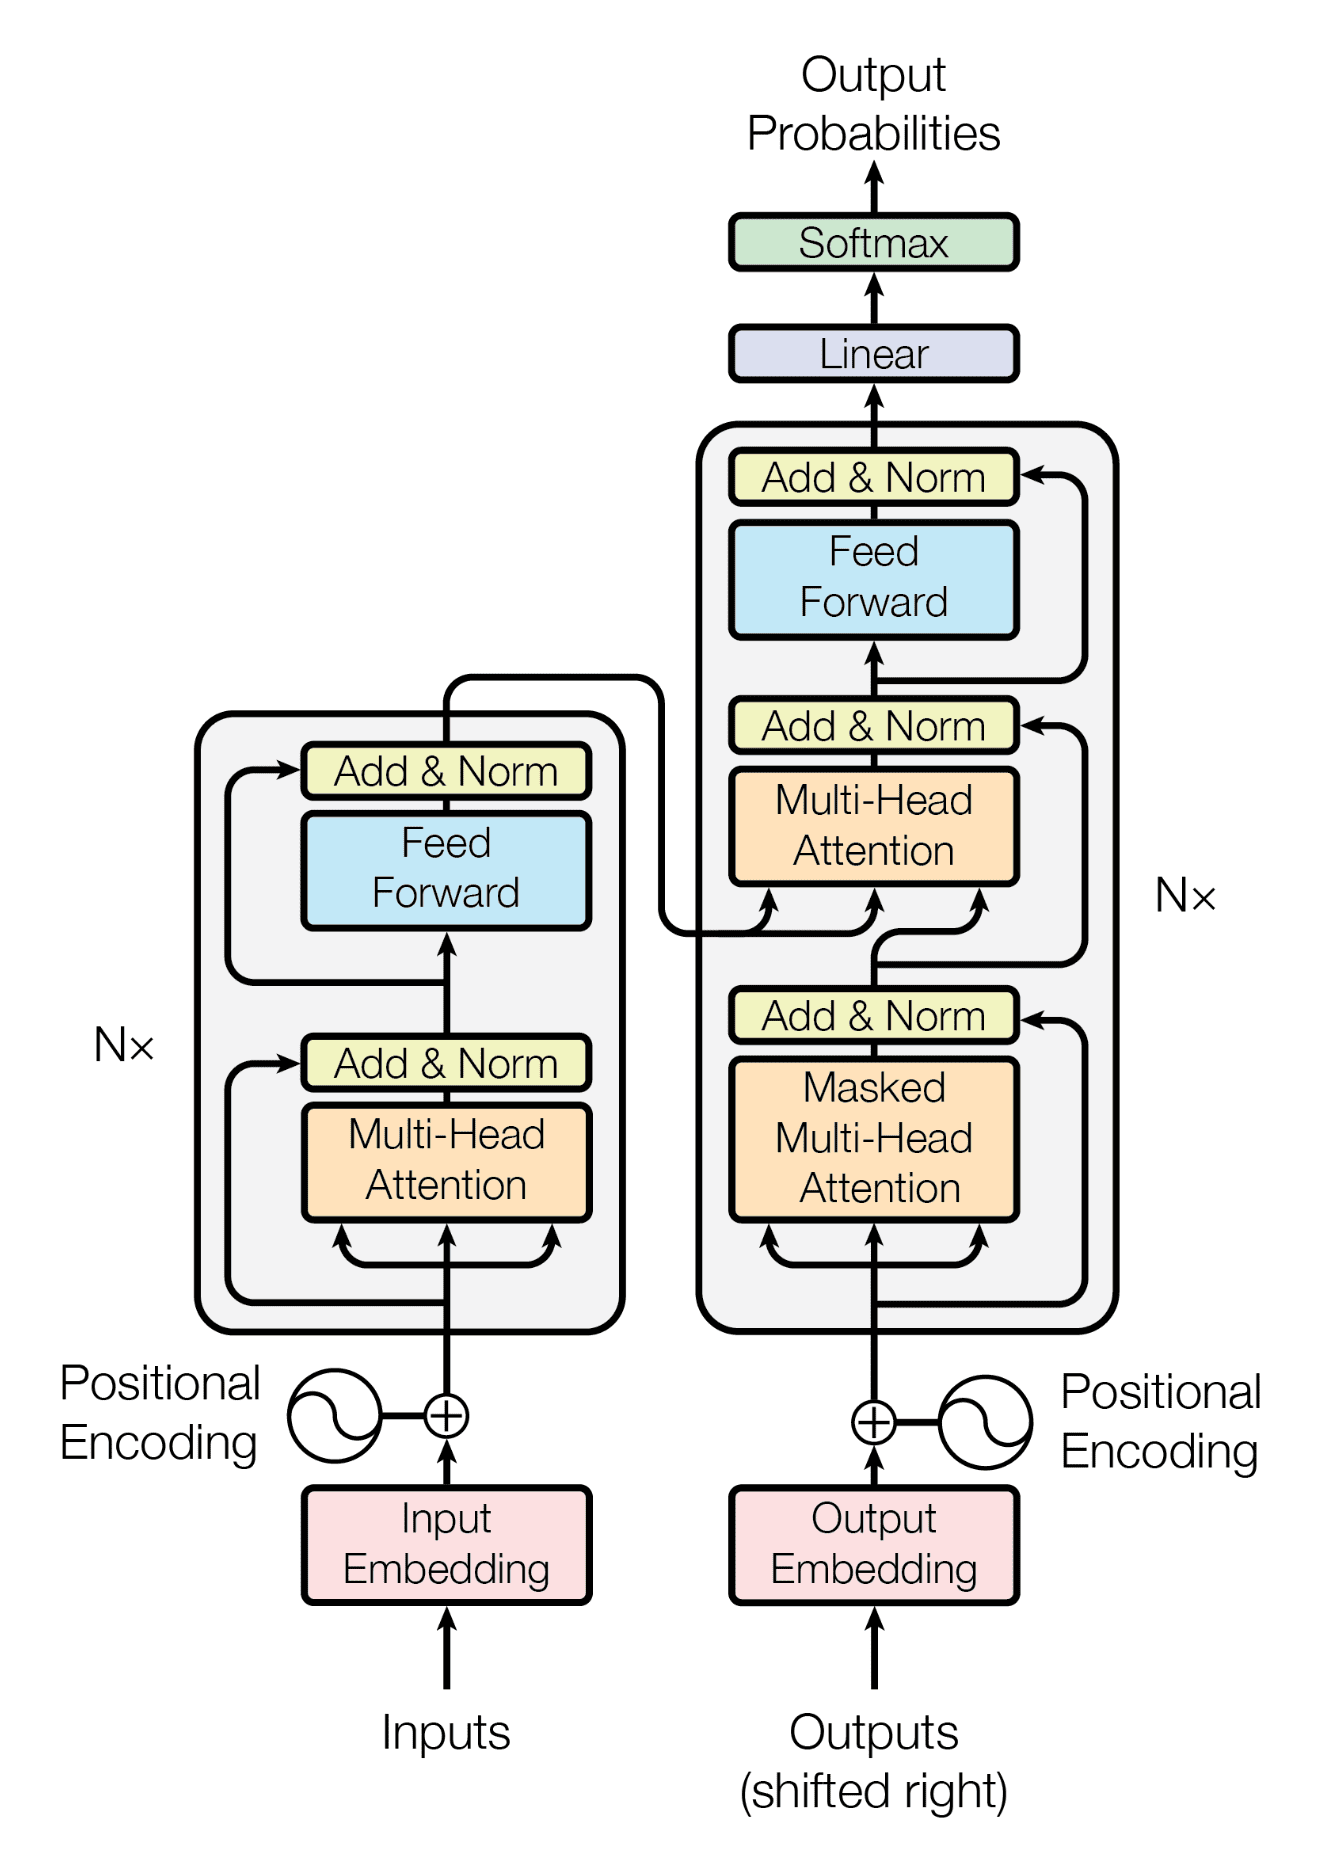
\includegraphics[width=0.6\linewidth]{docs/figs/transformer.png}
    \caption{Transformer architecture diagram \cite{attention_is_all_you_need}}
    \label{fig:transformer}
\end{figure}

As we can see, the architecture lends itself to parallelization, which in turn helps speed up training and inference, but also increases the model's complexity.

For our work, we will focus on Transformer encoder stacks (which we will call Transformers hereon forwards) with multi-head attention, as these can be used for sequence classification rather than machine translation or sequence modeling.

These Transformers, when used along a feed-forward layer and a softmax layer, can output $n$-class classification probabilities, which we will use to determine if a string belongs to a certain language, after being trained on a dataset composed of strings of balanced and unbalanced parentheses.

Albeit Transformers are known for their state-of-the-art performance on natural language processing tasks, they cannot process words as-is; these inputs need to be mapped to a vector space $\mathbb{R}^d$. To this effect, we will use Ströbl's definition of a \emph{word embedding}, $\text{WE}: \Sigma \rightarrow \mathbb{R}^d$ \cite{strobl2024formal}. 

\section{Attention}

The attention mechanism is the most important part of this architecture and will be the focus of our study. In short, this mechanism will let the model know the importance of a \emph{token} with respect to all other tokens in the sequence. 

According to Vaswani et al., attention functions can be described as mappings of queries and key-value pairs to an output, where queries, keys and values are all vectors belonging to a vector space $\mathbb{R}^n$, where $n$ is called the \emph{embedding} or \emph{representation} dimension. As defined above, Ströbl defines these vectors as mappings that stem from applying a length preserving function $f: \Sigma^* \rightarrow (\mathbb{R}^d)^*$ to input strings \cite{strobl2024formal}. This function consists of two components, the previously defined word embedding and a positional encoding, PE, such that:

\begin{equation}
    f(w_0\dots w_{n-1})_i = \text{WE}(w_i) +\text{PE}(i)
\end{equation}

The most commonly used attention mechanism is called scaled dot-product attention, which is defined as follows:

\begin{equation} \label{eq:attn}
    \text{Attention}(Q, K, V) = \text{softmax}\left( \frac{QK^T}{\sqrt{d_k}} \right)V
\end{equation}

In practice, $Q, K, V$ in equation \ref{eq:attn} refer to batched queries, keys and values respectively, where individual queries, keys and values are packed into matrices and processed simultaneously, speeding up computation.

Furthermore, this mechanism can be split and parallelized, which is then known as \emph{multi-head attention}, and represented by the following equation:
\begin{equation} \label{eq:multihead-attn}
    \begin{split}
        \text{MultiHead}(Q, K, V) &= \text{Concat}(\text{head}_1, \dots, \text{head}_n)W^O \\
        \text{where head}_i &= \text{Attention}(QW_{i}^{Q}, KW_{i}^K, VW_{i}^V)
    \end{split}
\end{equation}

In this mechanism, $W_{i}^{\{Q, K, V\}}$ are learned parameter matrices. Splitting the attention mechanism into different \emph{heads} allows for attending to information at different positions using different representations, without incurring in severe computational cost penalties, as the reduced dimensionality of each head allows for a computational cost similar to single-head attention with full dimensionality \cite{attention_is_all_you_need}.

We find this mechanism of interest for our work, as we believe attention will provide information regarding if a certain string of parentheses is balanced, and therefore, information about its membership to a $D_k$ language.
